\chapter{Experiments with DVI LCoS}
\begin{summary}
  Initially we strived to create a prototype, that would allow
  feedback between the spatial SLM and the camera with
  \unit[60]{Hz}. It was based on a fast ferroelectric liquid crystal
  on silicon device with DVI (digital video interface) data input as
  the spatial SLM.
  
  We overcame several problems with synchronization, latencies and
  light efficiency. Finally the remaining problems turned out to be
  too difficult to overcome\footnote{Retrospectively, there seems to
    be a solution which we mention in the discussion to this section.}
  and we rather switched to a spatial SLM solution with local storage
  as described in the main body in this work.

  Nevertheless we believe spatio-angular illumination with realtime
  control will be very useful and therefor we describe our system,
  even though it is impractical for now.
\end{summary}

\section{Description of the setup (fast MMA)}
The optical setup is the same as in \figref{fig:memi-real}. Sometimes
we use a blue LED diode array (CoolLed) instead of the laser as a
light source, that we couple with a fibre bundle into the integration
tunnel. The LED delivers less brightness but a more uniform
illumination -- especially of the MMA.

The ferroelectric LCoS display is nearly identical to the one used in
the main text (SXGA R3, ForthDD) but the data is transferred into the
controller from the computers graphics card via DVI. The computer
transmitts digital $24-$bit images ($1280\times1024$ pixels) with
$\unit[60]{Hz}$\footnote{Up to \unit[85]{Hz} are supported by the
  ferroelectric LCoS. This corresponds to a frame rate of
  $24\times\unit[85]{Hz}=\unit[2040]{Hz}$ of individual bit
  planes.}. The LCoS controller then displays a sequence of 24
bitplanes. Each bitplane is shown for $\unit[276.27]{\mu s}$ as
indicated in the $\verb!RED_ENABLE!$ signal in \figref{fig:trigger0}.

Originally the LCoS controller was designed by ForthDD to display
color images with 8 bits per color. In order to do this it would
display three times eight images of pulses, where each pulse would be
half the length of its predecessor. Three separate galvanically
decoupled TTL signals would then enable corresponding LEDs for red,
green and blue. We use the controller in a modified mode (48366
BitSlice 768-line 60Hz V1.0), where it would display each bitplane for
equal amounts of time and generate all light enable pulses on
\verb!RED_ENABLE!.

Unfortunately the company doesn't provide the vertical sync signal
(which is generated by the graphics card in the computer). As a remedy
we use a microcontroller (Arduino) program (see code listing on page
\pageref{fig:arduino-vsync}), that reads the \verb!RED_ENABLE! signal,
counts the pulses and measures the time between them. This way we are
able to find the longer gap of $\unit[587]{\mu s}$ infront of the
first pulse (which corresponds to bit 0 of the red byte).

% /home/martin/from-hp2-notebook/Downloads_pdf/Downloads4/Downloads/48366_BitSlice_768-line_60Hz.pdf

Initially we planned our device to run at the fastest possible
speed. The MMA has a delay of $\unit[850]{\mu s}$ between receiving a
trigger edge and the mirrors having settled in the requested
orientation. In order to run the MMA at a fast frame rate we decided
to generate a trigger pulse in the Arduino microcontroller after every
second LCoS bitplane. This gives enough time to the MMA controller to
set the mirrors and we can display simultaneous images on MMA and LCoS
during 11 out of 24 LCoS bitplanes. The system therefor achieves a
frame rate of $\unit[60]{Hz}\times11=\unit[660]{Hz}$ and a duty cycle
of just $\unit[277]{\mu s}\times11\times\unit[60]{Hz}=0.18$.

\section{Description of the trigger generation (slow MMA)}
We should note, that the MMA is a prototype as well and its
controller, though being connected to the computer via ethernet,
doesn't support \unit[1]{Gbit/s} communication or any other means that
would allow realtime update of its image, e.g. support for run-length
encoding of the image data. Therefor the MMA can display images with
\unit[660]{Hz} but uploading one new image roughly takes
\unit[80]{ms}.

It therefor seems reasonable to switch to a different mode, where the
mirrors of the MMA are tilted for one full video frame. The MMA has a
limited maximum duty cycle of 50\%. This means we have to drop every
other frame from the graphics card. If camera exposure times of
\unit[16.66]{ms} are sufficient, we can even increase the duty cycle
of the full system to $\unit[277]{\mu
  s}\times24\times\unit[60]{Hz}=0.4$.


{\small\label{fig:arduino-vsync}
\begin{verbatim}
// takes the lcos signal (train of 24 pulses, followed by a pause)
// and generates a trigger signal for the mma at the end of each train
// so for every DVI image (consisting of 24 bit planes) a different
// mma image can be shown. 

volatile unsigned int Ticks;    // holds the pulse count as .5 us ticks
// pin 8 takes signal from lcos
char icpPin = 8;                // this interrupt handler must use pin 8
volatile char bit_plane_change = 0;  // incremented whenever a 
                                     // different bitplane is displayed
char mma = 13;                  // output towards mma

ISR (TIMER1_CAPT_vect) // interrupt gets called when pin 8 changes
{
        if (!bit_is_set (TCCR1B, ICES1))        // was rising edge detected?
                TCNT1 = 0;      // reset the counter
        else {                  // falling edge was detected
                Ticks = ICR1;
                if (Ticks > 1000) {
                        bit_plane_change = 0;
                }
        }
        TCCR1B ^= _BV (ICES1);  // toggle bit value to trigger on the
                                // other edge
        if (bit_plane_change == 47) {
                digitalWrite (mma, HIGH);
        }
        else if (bit_plane_change == 0) {
                digitalWrite (mma, LOW);
        }
        bit_plane_change++;
}
void setup ()                   // run once, when the sketch starts
{
        pinMode (icpPin, INPUT);
        pinMode (mma, OUTPUT);
        TCCR1A = 0x00;          // COM1A1=0, COM1A0=0 => Disconnect Pin OC1
                                //                     from Timer/Counter 1
                                // PWM11=0,PWM10=0 => PWM Operation disabled
        TCCR1B = 0x02;          // 16MHz clock with prescaler means TCNT1
                                // increments every .5 uS (cs11 bit set)
        Ticks = 0;              // default value indicating no pulse detected
        TIMSK1 = _BV (ICIE1);   // enable input capture interrupt for timer 1
}
int getTick ()
{
        int akaTick;            // holds a copy of the tick count so we can
                                // return it after re-enabling interrupts
        cli ();                 // disable interrupts
        akaTick = Ticks;
        sei ();                 // enable interrupts
        return akaTick;
}
char get_plane_change ()
{
        int aka;
        cli ();
        aka = bit_plane_change;
        sei ();
        return aka;
}
void loop () {}                 
\end{verbatim}
}

\begin{figure}[!hbt]
  \centering
  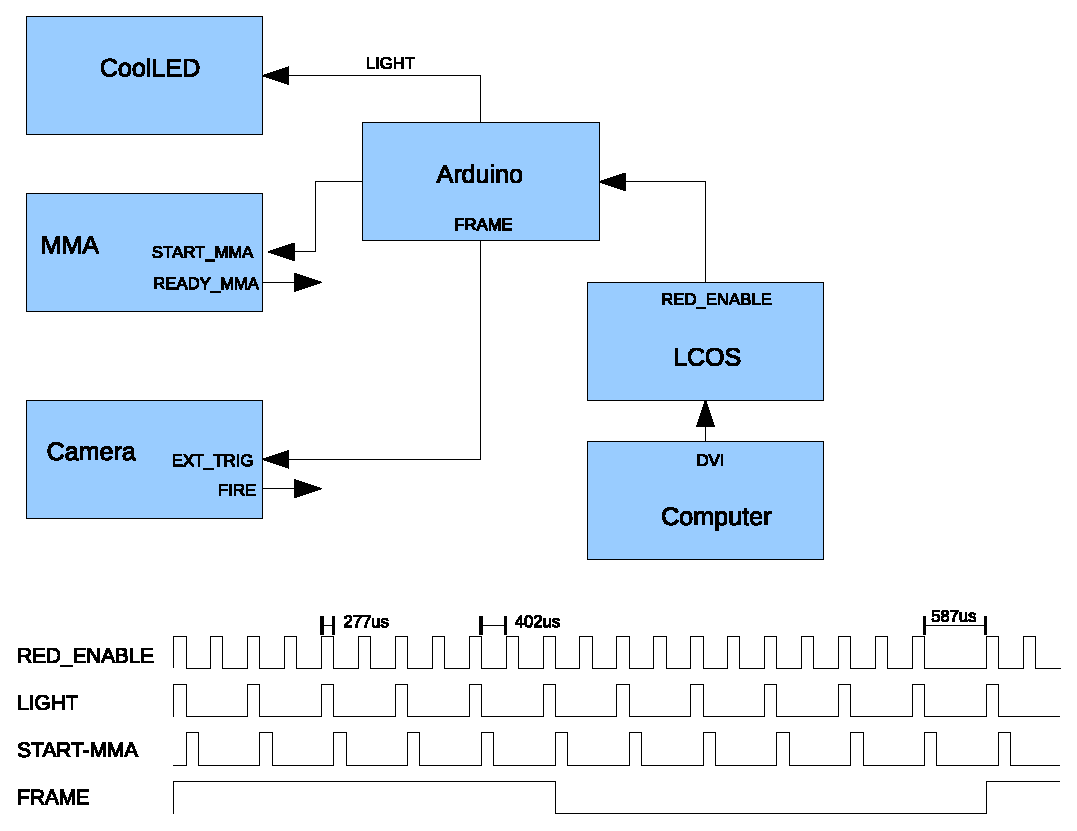
\includegraphics[width=14cm]{../dvi/trigger0}
  \caption{{\bf top:} Schematic of the electronic components of the
    system and how they are connected. {\bf bottom:} Depiction of TTL
    trigger signals for the ``fast MMA'' configuration.}
  \label{fig:trigger0}
\end{figure}


\begin{figure}[!hbt]
  \centering
  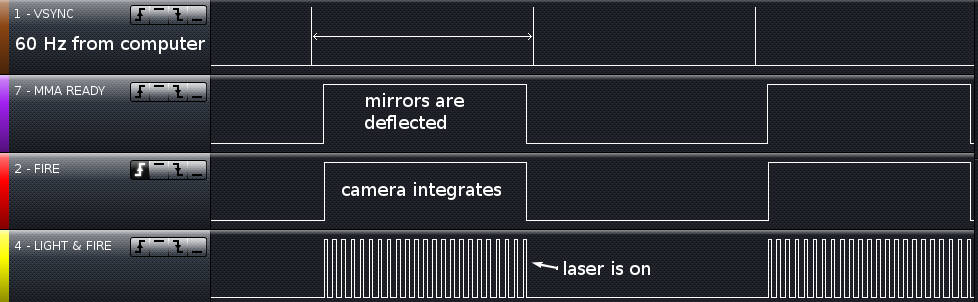
\includegraphics[width=12cm]{screen_logic_labels}
  \caption{Snapshot of the trigger signals for the ``slow MMA''
    configuration with a logic analyzer (Saleae Logic).}
  \label{fig:screen_logic_labels}
\end{figure}

\begin{figure}[!hbt]
  \centering
  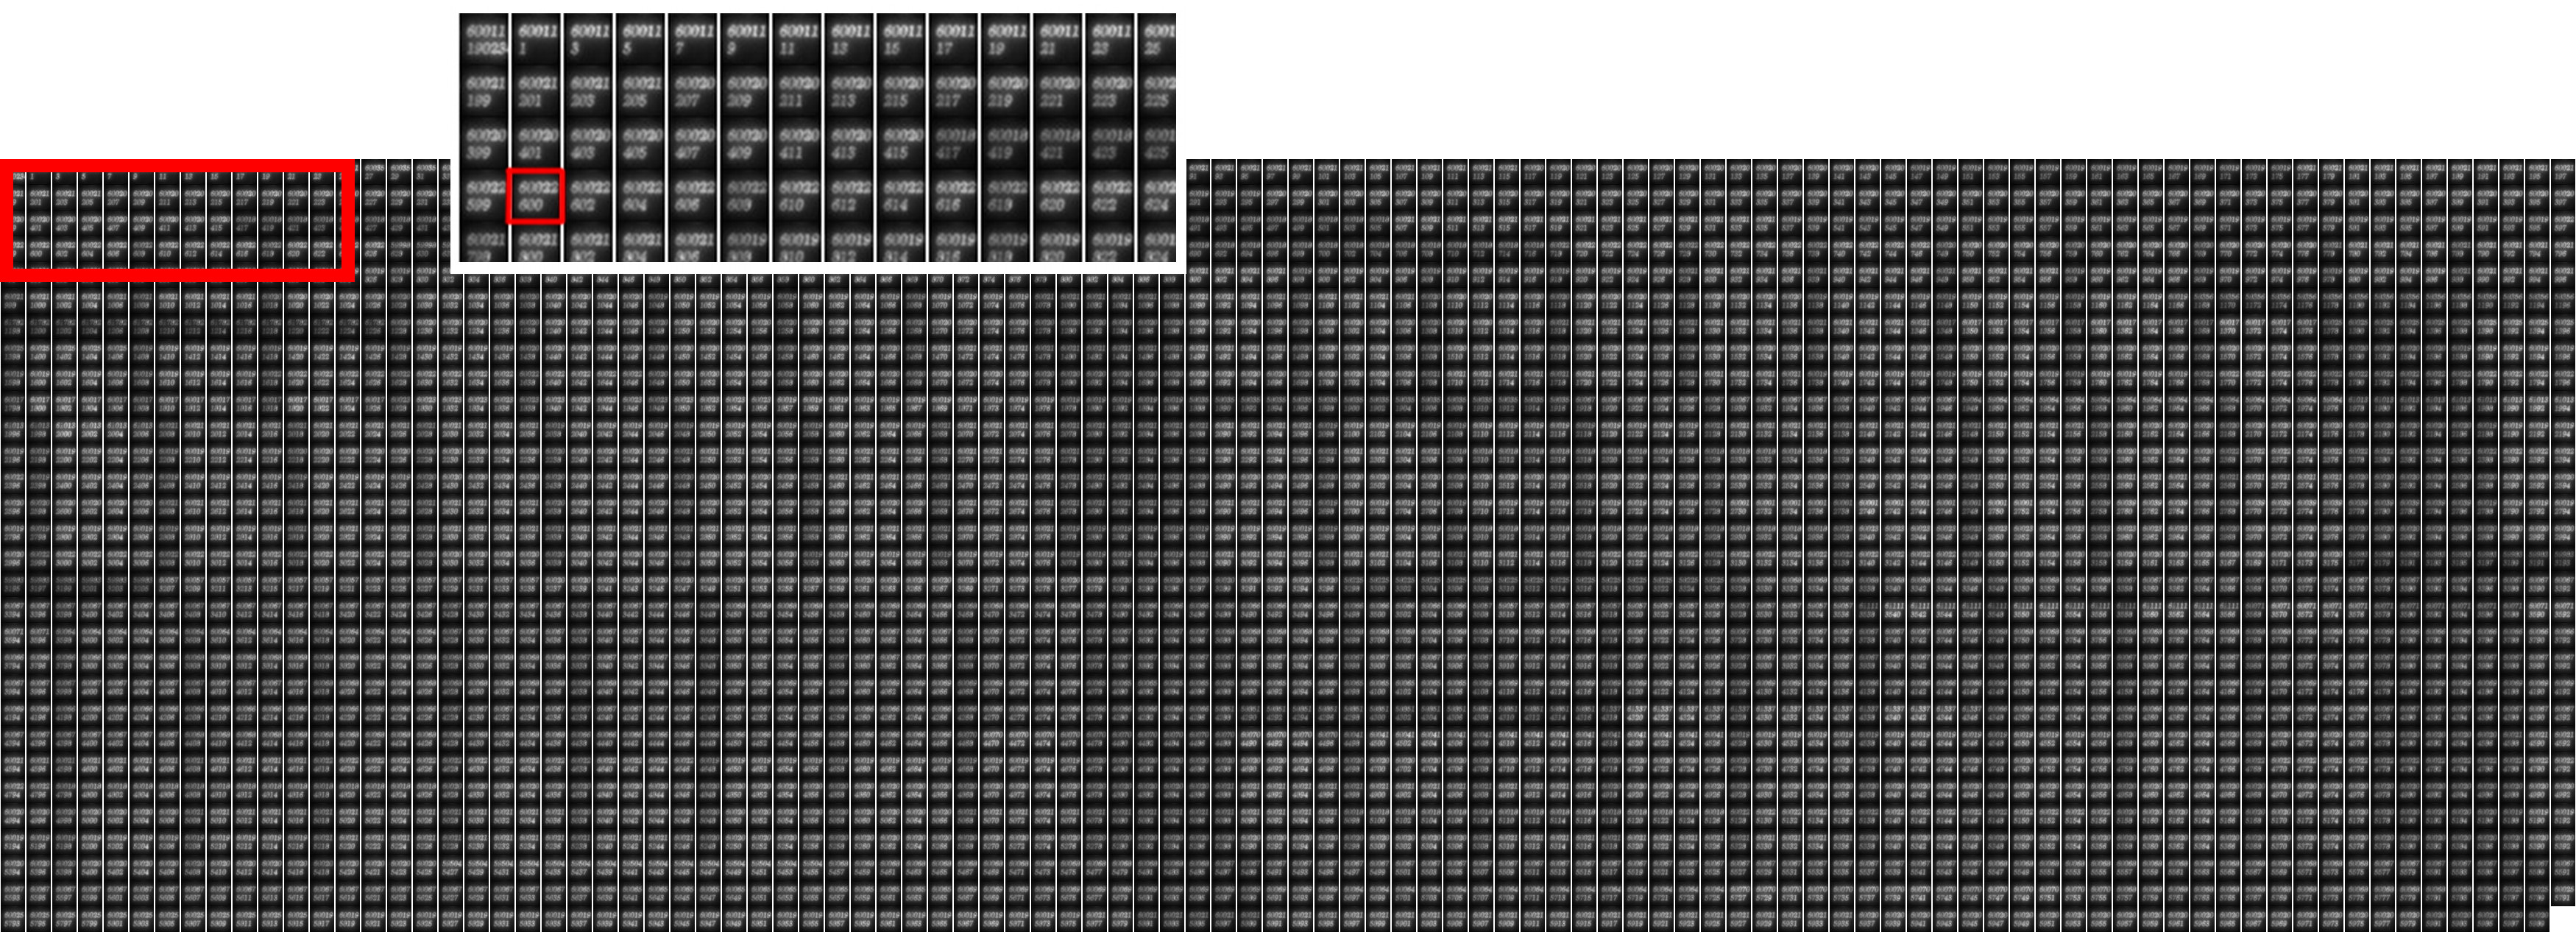
\includegraphics[width=14cm]{fast4-no-first_cut}
  \caption{}
  \label{fig:fast4-no-first_cut}
\end{figure}


\begin{figure}[!hbt]
  \centering
  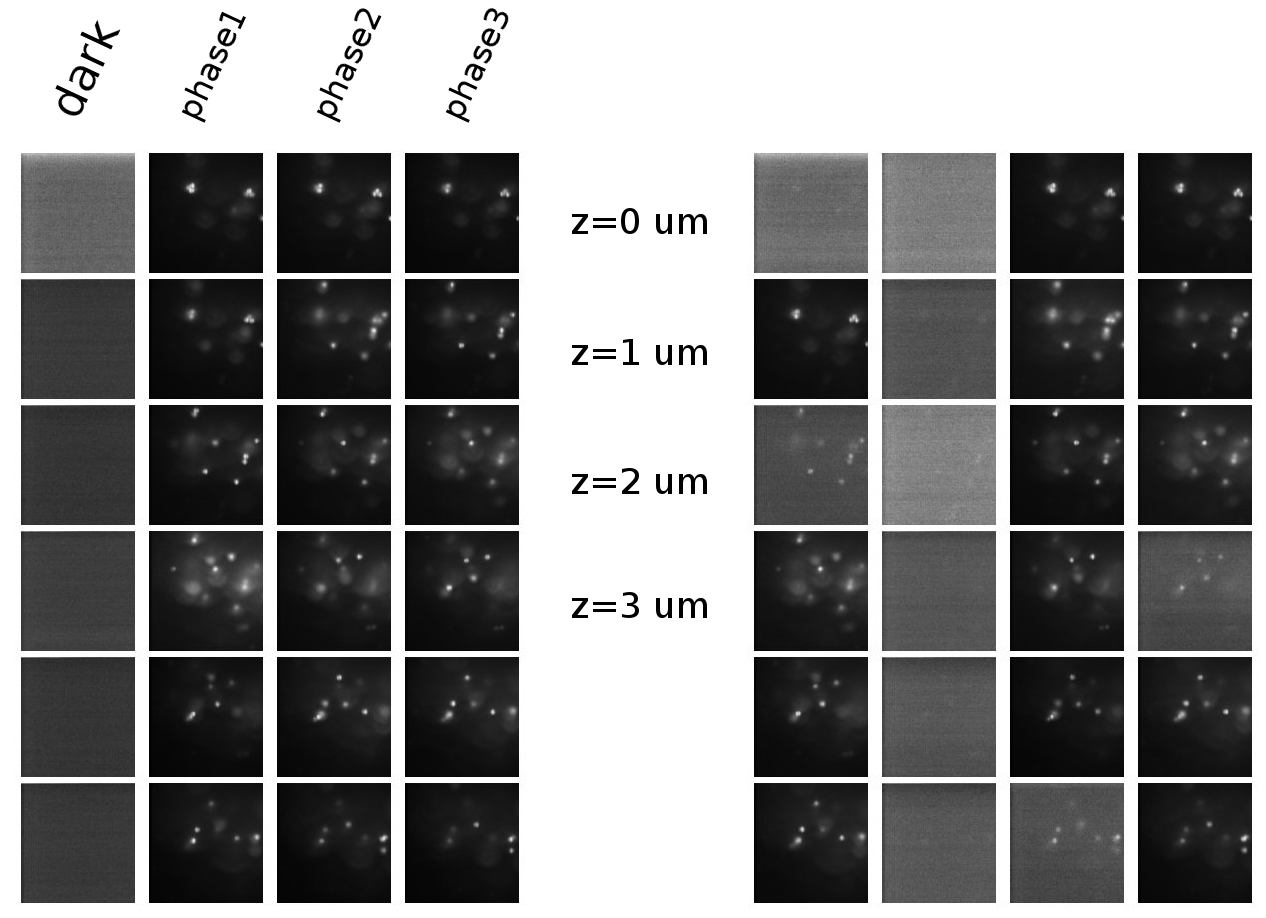
\includegraphics[width=10cm]{dvi-mosaic}
  \caption{{\bf left:} Sequence of images that was aquired while LCoS,
    MMA, z-stage and camera are running in sync. The camera is
    constantly running at \unit[30]{Hz} and the stage moves while a
    black mask is displayed on the MMA as well as the LCoS.}
  \label{fig:dvi-mosaic}
\end{figure}

